\documentclass{beamer}

\usepackage{animate}
\usepackage{subfigure}
\usetheme{AnnArbor}
\usecolortheme{beaver}


\title 
{Feature Extraction and Classification of Plankton}
\subtitle
{ We done things }
\author{Dane Skinner \and Nick Hockensmith \and Kevin Park}
\institute
{Oregon State University}
\date
{May 15, 2014}


\begin{document}
\begin{frame}
	\maketitle
\end{frame}
%----------------------------------
% FRAME 2
%----------------------------------
%\begin{frame}
%\frametitle{Outline}
%	\begin{itemize}
%	\item Question of Interest
%	\item Feature Extraction
%	\item Classification Models: Random Forest \& kNN 
%	\item Conclusion and Final Thoughts
%	\end{itemize}
%\end{frame}

%----------------------------------
% FRAME 3
%----------------------------------

\begin{frame}
\frametitle{Questions of Interest}
\begin{itemize}
	\item Using Histogram and Image Moments as a image feature extraction how accurate are the classification of plankton?
%	\item Does a change in the environment effect our predictions?
\end{itemize}

\end{frame}

%----------------------------------
% FRAME 5
%----------------------------------

\begin{frame}
\frametitle{Kratuchok's Moments}
$\bullet$ Calculating \textit{Kratuchok's} moments,
\begin{equation*}
Q_{nm} = \sum_{x=0}^{N-1}\sum_{y=0}^{M-1}\bar{K}_n(x;p_1,N-1)\bar{K}_m(y;p_2,M-1)f(x,y),
\end{equation*}
where  $f(x,y)$ is the pixel intensity and ($K_n(a;p,N$) are the weighted Krawtchouk polynomials, and $n\in \mathbb{N}$ is order of the moment in the x- or y-direction.\\
$\bullet$ Kratuchok moments are invariant under scaling, rotation, and translation. \\
\end{frame}

%----------------------------------------------------------------
% FRAME 5.5
%----------------------------------------------------------------

\begin{frame}
\frametitle{Kratuchok's Moments}
$\bullet$ The training set was further divided into a training and validation set to determine the order of moments that yielded the ``best" classification of the validation set. \\
$\bullet$ As you can see below, it appears that the $6^{th}$ moment offers the best prediction of the validation set.
	\begin{center}
		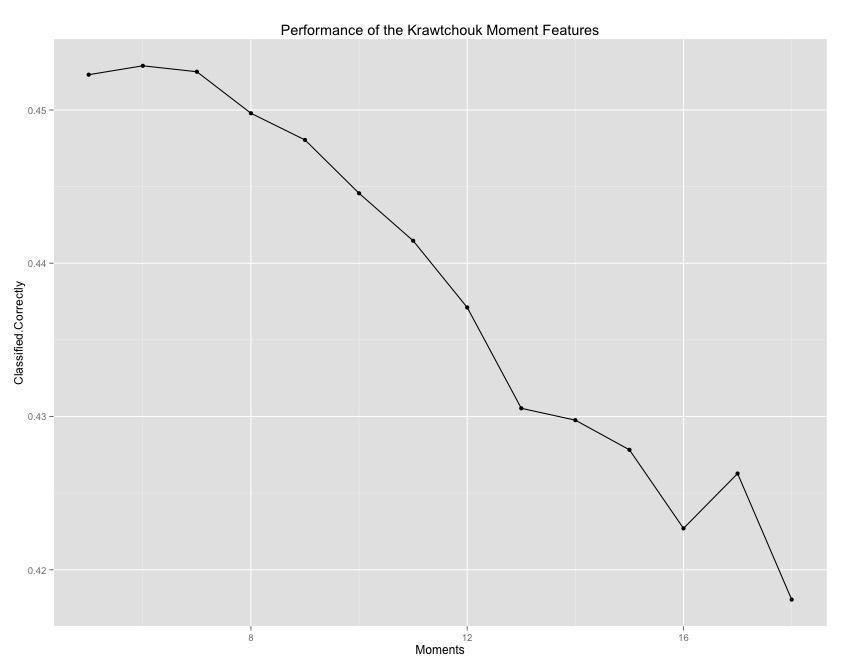
\includegraphics[scale=0.20]{norasta.jpeg}
	\end{center}
\end{frame}

%----------------------------------
% FRAME 6
%----------------------------------

\begin{frame}
\frametitle{Histogram Method}
$\bullet$ Some of species of plankton give distinct distributions of gray scale values. 
\begin{center}
	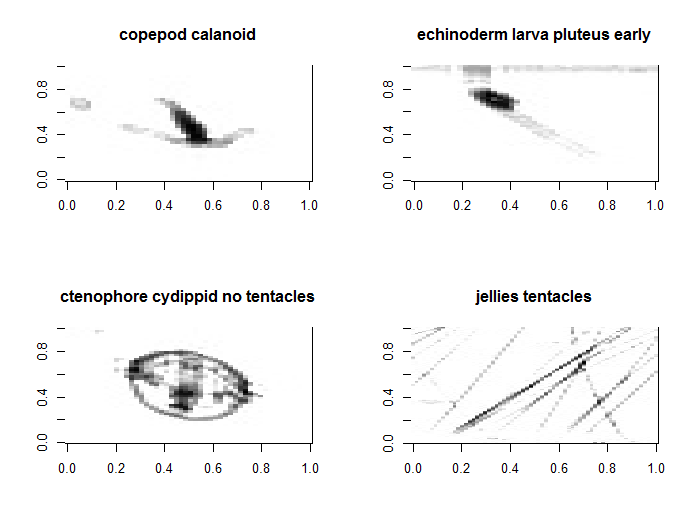
\includegraphics[scale=0.23]{images.png}
	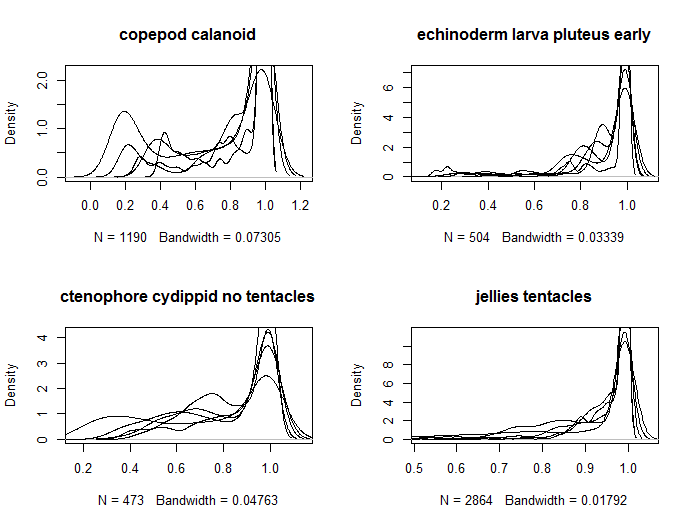
\includegraphics[scale=0.23]{grayscale.png}
\end{center}
\end{frame}

\begin{frame}
	\frametitle{Histogram Method}
	$\bullet$ The grayscale is on a [0,1] interval and we partition the interval into a width of 0.1.\\
	$\bullet$ We have count the number of values that are between $[0,0.1],[0.1,0.2],\cdots, [0.9,1]$.\\ 
	\begin{center}
		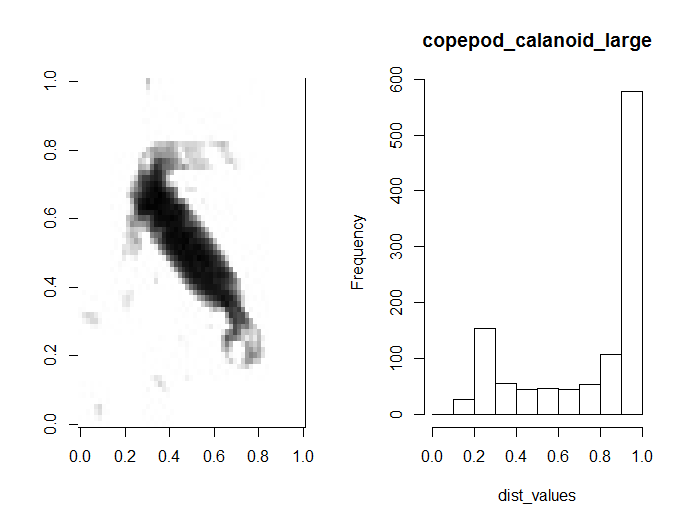
\includegraphics[scale=0.3]{bin_method.png}
	\end{center}
\end{frame}
%----------------------------------
% FRAME 7
%----------------------------------
\begin{frame}
	\frametitle{Indicoio Package and kNN}
$\bullet$ This produces a sparse, 2048 digit feature vector for each image that can then be used to calculate the Euclidean distances between different feature vectors.\vskip 12pt

$\bullet$ The data extracted from Indicoio was too "noisy" for kNN to make any accurate classifications and the large number of classes made it difficult for computation time. \vskip 12pt

$\bullet$ The kaggle score was 8.1 ($\sim$1001 ranking).

\end{frame}

%----------------------------------------------------------------
% FRAME 8.25
%----------------------------------------------------------------

\begin{frame}
	\frametitle{Kaggle Results: Histogram \& Momements}
$\bullet$ We were fairly surprised at some of our results.\\
$\bullet$ Histogram method produced a score of 3.29. \\
\begin{center}
	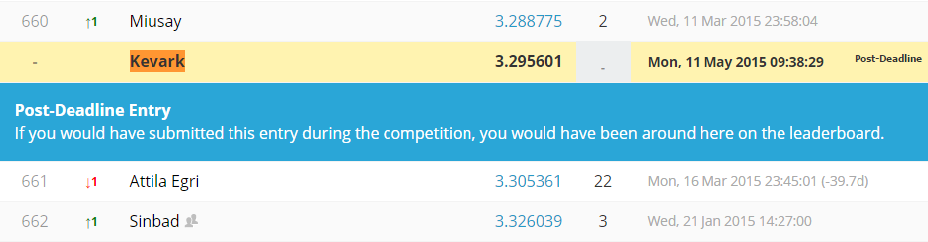
\includegraphics[scale=0.3]{submission.png}
\end{center}
$\bullet$ Combination of Histogram and $10^{th}$-order Krawtchouk scored 2.66\footnotemark. \\
\begin{center}
	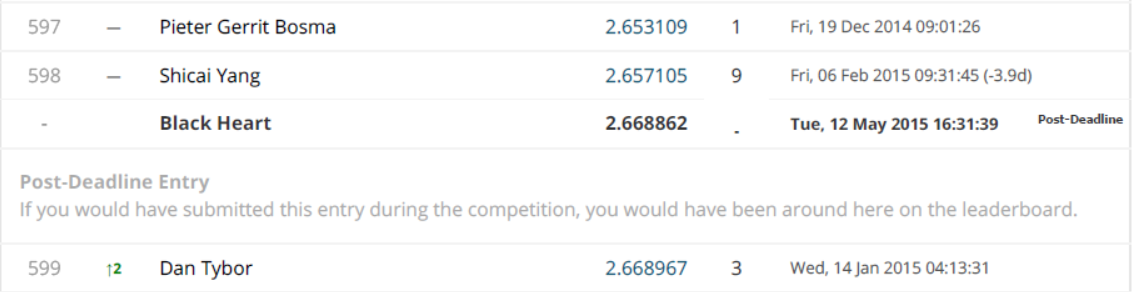
\includegraphics[scale=0.25]{combined.png}
\end{center} 

\footnotetext[1]{readJPEG not set to default}

\normalsize
\end{frame}

%----------------------------------------------------------------
% FRAME 8.5
%----------------------------------------------------------------

\begin{frame}
	\frametitle{Kaggle Results:}
$\bullet$ $20^{th}$-order Krawtchouk moments produced a score of 2.18. \\
\begin{center}
	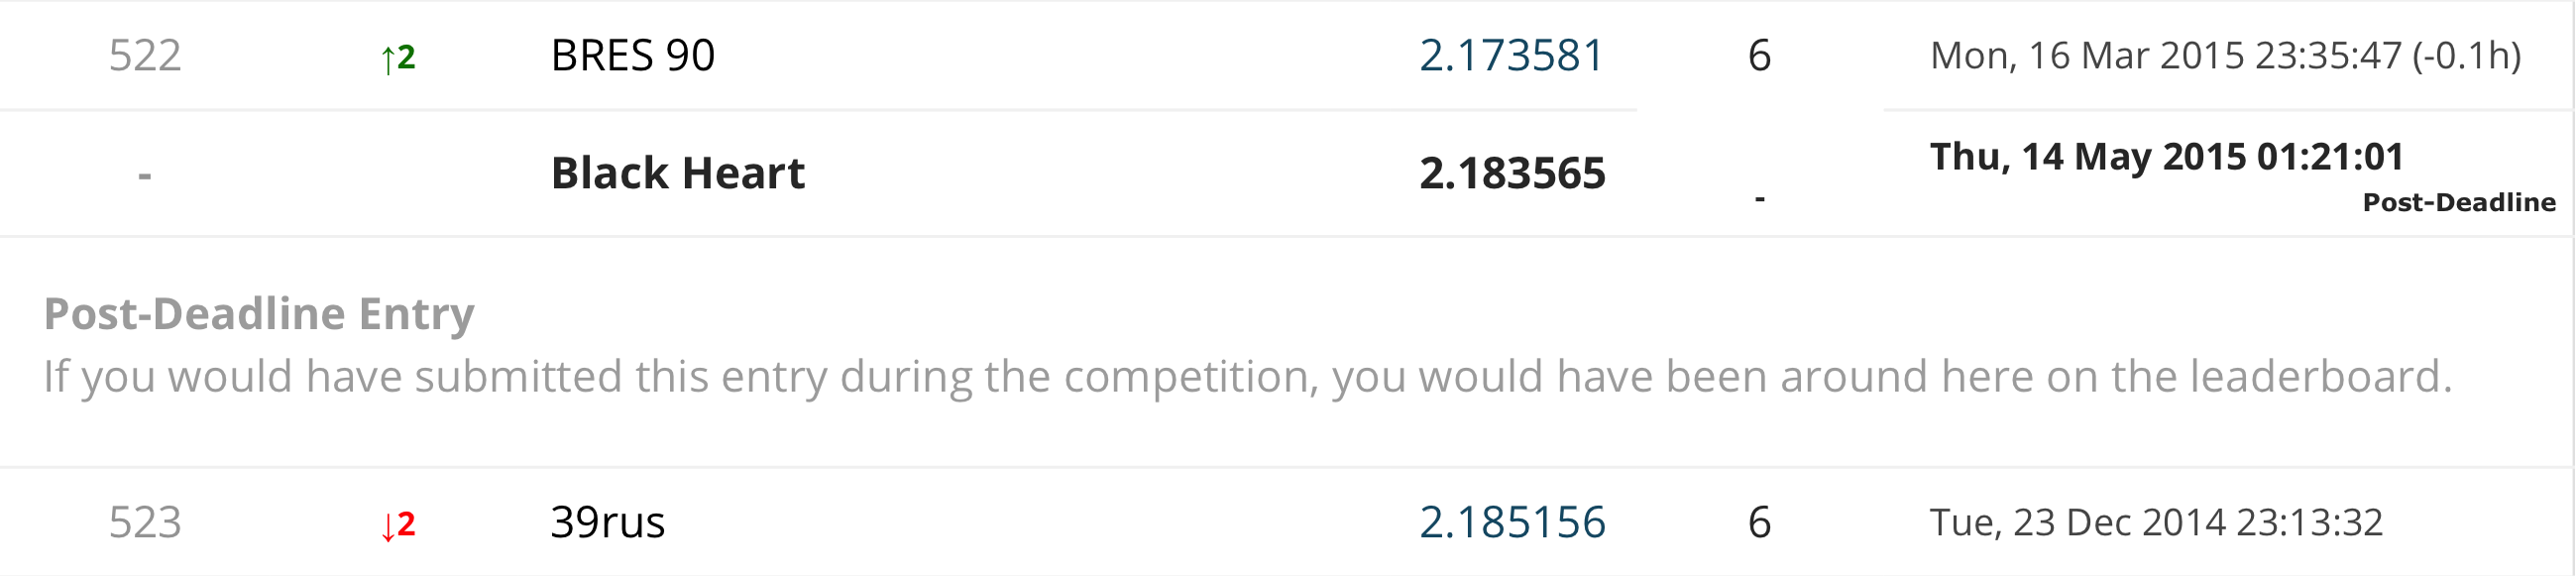
\includegraphics[scale=0.2]{Telly.png}
\end{center}
$\bullet$ Histogram and $6^{th}$-order Krawtchouk combo produced a score of 2.13. \\
\begin{center}
	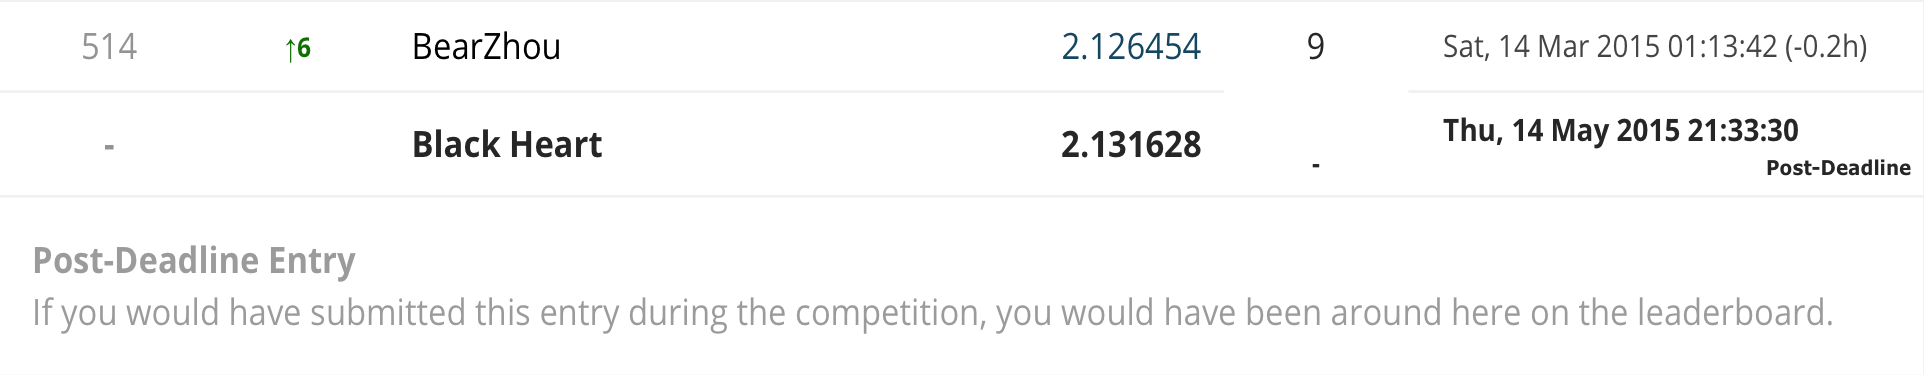
\includegraphics[scale=0.27]{KrawtBin6Mom.png}
\end{center}
\end{frame}

%----------------------------------------------------------------
% FRAME 9 
%---------------------------------------------------------------

\begin{frame}
	\frametitle{Conclusions and Final Thoughts}
	\begin{itemize}
		\item Krawtchouk moments required 400 features to achieve it's best Kaggle rank of 523/1049.
		\item The Histogram method required only 10 features to achieve it's best Kaggle rank of 661/1049.
	\end{itemize}
As future work, 
	\begin{itemize}
		\item Perform variable selection for dimension reduction on the Krawtchouk moments.
		\item Increase the number of bins measured in the Histogram method.
		\item Look towards 2-D filters for additional features.
	\end{itemize}
\end{frame}

\end{document}
